%----------------------------------------------------------------------------
\chapter{Valószínűségelmélet}
%----------------------------------------------------------------------------

Az alábbi fejezetben a Bayes-tétel és annak következményei szerepelnek. Ezek ismerete szükséges a Diplomamunka központi algoritmusának megértéséhez.

\section{Bayes-tétel}
Jelölje az A esemény bekövetkezésének valószínűségét $P(A)$, $AB = A \cap B$ azt az eseményt, amikor A és B is bekövetkezik, és $P(A|B)$ az A feltételes valószínűségét B-re nézve. Ha A és B független események a feltételes valószínűség definíciójából következik, hogy
$$P(AB) = P(A \cap B) = P(A|B) \cdot P(B) =  P(B|A) \cdot P(A) $$
Ebből egy osztással megkapható a tétel állítása
$$P(A|B) = \frac{P(B|A) \cdot P(A)}{P(B)}$$
amely segítségével egy feltételes valószínűség az események valószínűsége és az ellenkező irányú feltételes valószínűség ismeretében meghatározható. Tehát van a feltételes valószínűségek között egy megfordíthatóság \cite{laszlo2011bayesi}.

B esemény felbontható a $\{A_i\}$ teljes eseményrendszerre, vagyis a $P(A_i \cap A_j) = 0$, ha $i \neq j$ és $ P(\bigcup_{i} A_i) = 1$. Ez azt jelenti, hogy az eseményteret olyan eseményekre bontjuk, amelyek közül minden esetben pontosan egy következik be és az egyik közülük mindenképpen bekövetkezik. Ilyenkor is alkalmazható marad a \emph{Bayes-tétel}:
$$P(A_i|B) = \frac{P(B|A_i) \cdot P(A_i)}{\sum_{j} P(B|A_j) \cdot P(A_j)}$$
Eszerint ha egy teljes eseményrendszer valószínűségei és hozzá kapcsolódóan egy másik B esemény feltételes valószínűségei ismertek, akkor meghatározható az eseményrendszer eseményeinek a B eseményhez tartozó feltételes valószínűségei.

\section{Bayes-háló}
A teljes eseményrendszerek közötti kapcsolatok irányított gráf formában is ábrázolhatók. A gráfban a csomópontok a teljes eseményrendszerek az élek pedig a közöttük lévő közvetlen összefüggéseket reprezentálja. Ilyenkor az élek irányának nincs különösebb jelentősége. Az így felépített irányított körmentes gráf egy \emph{Bayes-háló}. A körmentesség abból adódik, hogy csak a közvetlen összefüggések vannak éllel jelölve, így nem tud bezárulni egy kör, mert a két változó közt nem lehet egyszerre áttételes és direkt függés is.

A reprezentáció értelmezése kiterjeszthető. Egyrészt az eseményrendszerek helyett a csomópontokba beilleszthetők valószínűségi változók is. Másrészt az élek menti kapcsolatokat súlyozhatjuk a két valószínűségi változó feltételes valószínűségeivel, amelyben a kiindulópontra vonatkozik a célpontnak a feltételes valószínűsége. Az irány emiatt fontossá válik, az él megfordításakor a Bayes-tétellel számolható ki az ellentétes irányú feltételes valószínűség.

Így a Bayes-háló alkalmassá válik tudásreprezentációra is. Ebben az értelmezésben az élek iránya ok-okozati összefüggést mutat. A háló felépítése szakértőre vagy egy szakértői rendszerre van bízva. Ilyenkor a szakértő megkötéseket tehet, milyen kapcsolatok kell teljesüljenek vagy nem teljesülhetnek, valamint a valószínűségekre és feltételes valószínűségekre is adhat becslést vagy rögzítheti azokat.

\begin{figure}[htp]
    \centering
    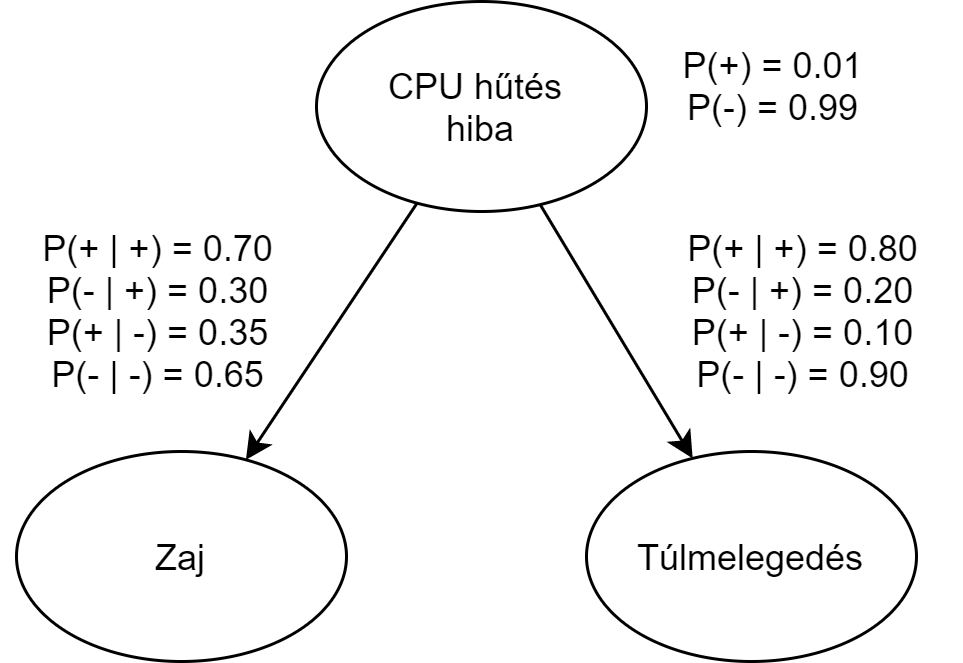
\includegraphics[width=12cm]{figures/BayesianNetwork.png}
    \caption{Tudásreprezentáció Bayes-hálóval}
    \label{fig:bayes-halo-tudasrep}
\end{figure}

Emellett ismert adatsorok alapján is felépíthetők ilyen rendszerek. Jelen Diplomamunka célja egy olyan könyvtár készítése, mely egy statisztikai adatsor alapján építi fel a tudásreprezentációra szolgáló Bayes-hálót.

A \ref{fig:bayes-halo-tudasrep} ábrán látható, hogyan használható a Bayes-háló tudásreprezentációra. Egy számítógép processzorának meghibásodását, és annak jeleit modellezi. A valószínűségi változók ebben az esetben binárisok, a + jelöli az igaz értéket. A processzor meghibásodásának valószínűsége 1\%. Annak a valószínűsége, hogy nem hibásodott meg, értelemszerűen $100\%-1\%=99\%$. Látható, hogy a $P(-)$\footnote{Ez egy egyszerűsített jelölésmód. Az X valószínűségi változóra a $P(+)$ azt a valószínűséget jelzi, hogy X igaz értéket vesz fel, tehát $P(+) = P(X=+) = P(X=True)$. Amikor egyértelmű, mely változóra vonatkozik a jelölés, ebben a Diplomamunkában az első jelölésmódot alkalmazom.}, $P(-|+)$, $P(-|-)$ kifejezések felírása redundáns, mivel a $+$ párjaikat 1-re egészítik ki.

Szintén leolvashatók a feltételes valószínűségek értékei. Például annak a valószínűsége, hogy Zaj keletkezik, amennyiben a processzor hűtése nem hibás, azt a bal oldali táblázat $P(+|-)$ valószínűségeként találjuk meg, ami 35\%.

A \emph{Zaj} és \emph{Túlmelegedés} változók határeloszlása\footnote{A változó igaz és hamis értékének valószínűsége. Például a Zaj változóra P(+).} szintén redundáns információ, ezek nem is szerepelnek az ábrán. Ezek a Bayes-hálóban történő következtetéssel számolhatók ki. Annak a valószínűsége, hogy hallunk zajt, miközben a másik két változóról nem tudunk semmit, kiszámolható a CPU hűtés hiba és a feltételes valószínűségek szorzatai összegéből.
$$P(Z=+) = P(Z=+\,|\,C=+) \cdot P(C=+) + P(Z=+\,|\,C=-) \cdot P(C=-) =$$
$$= 0.7 \cdot 0.01 + 0.35 \cdot 0.99 = \textbf{0.3535} $$
A CPU hűtés hiba valószínűségi változót C, a Zaj-t Z jelöli. A nem hallható zaj valószínűségéhez innen kétféleképpen is eljuthatunk. A fenti képletet alkalmazzuk a nem hallható zajra vagy 100\%-ból kivonjuk a Zaj valószínűségét.
$$P(Z=-) = 0.3 \cdot 0.01 + 0.65 \cdot 0.99 = \textbf{0.6465} = 1-0.3535 $$

A Zaj-ból a processzor túlmelegedésére következtetés a Bayes-tétel alapján történhet.
$$P(C=+\,|\,Z=+) = \frac{P(Z=+\,|\,C=+) \cdot P(C=+)}{P(Z=+)} = \frac{0.7 \cdot 0.01}{0.3535} \approx \textbf{0.0198}$$
Ehhez hasonlóan a Bayes-hálóban bármely változó rögzítése esetén a többire valószínűség számolható.

% TODO: Háló elemei, elnevezések

\section{Becslés}
A valószínűségek segítségével becsléseket is adhatunk arra vonatkozóan, hogy a megfigyelések mellett mely állapot a legvalószínűbb. Ezek általánosan használhatók paraméterezhető modellekre.

\subsection{Legnagyobb valószínűség módszer}
Ez a módszer intuitívan adódik. Maximális valószínűséget keres az adott megfigyelt adatokhoz. Azt vizsgálja, hogy a lehetséges paraméterezések ($\Lambda$) közül melyik mellett a legnagyobb a megfigyelt adat ($D$) valószínűsége.
$$\argmax_{\Lambda}{P(D\,|\,\Lambda)}$$
A maximumkereséshez a valószínűség negatív logaritmusát lehet venni, így numerikusan stabilabb lesz, és ennek keresni a minimumát. Minimumkeresésre több módszert ismerünk, például a deriváltjának nullhelyét keressük. Ez a módszer jól alkalmazható, ha a modell felírható függvényként, és nem áll rendelkezésünkre előzetes ismeret a paraméterekről, csak a modell és a megfigyelések.

\subsection{Bayes-döntés}
Amennyiben van további ismeretünk a paraméterekről, úgy alkalmazhatunk olyan becslést, amely ezt figyelembe veszi. A Bayes-tétel segítségével vizsgálható a megfigyelt adathoz tartozó legvalószínűbb paraméterezés is, hiszen
$$\argmax_{\Lambda}{P(\Lambda\,|\,D)} = \argmax_{\Lambda}\{P(D\,|\,\Lambda) \cdot P(\Lambda)\}$$
Ennek a becslés típusnak a neve \emph{Bayes-döntés}, más néven \emph{a postreriori} vagy \emph{posterior becslés}. A negatív logaritmus minimalizálása itt is jó megoldás. A Legnagyobb valószínűség módszerben (maximum likelihood) szereplő tényezőt - $P(D\,|\,\Lambda)$ - \emph{likelihood} tagnak, az előzetes ismeretet tartalmazót - $P(\Lambda)$ - \emph{prior} tagnak nevezik. A tag elnevezés a gyakori negatív logaritmizálás miatt van, mert annak hatására a szorzatból összeg lesz, melynek ezek a tagjai.
